\synctex=1
\documentclass[11pt, a4paper]{article}

%% Packages
\usepackage{subcaption}
\usepackage{amsthm}
\usepackage{amsmath}
\usepackage{amsfonts}
\usepackage{booktabs}
\usepackage{natbib}
\usepackage{hyperref}
% \usepackage{fullpage}
\usepackage{graphicx}
\usepackage{mathtools}
\usepackage{color}
\usepackage[left = 2.5cm, right = 2.5cm, bottom = 3cm, top = 2.5cm]{geometry}
\usepackage{enumitem}
\usepackage{multirow}
\usepackage{rotating}
\usepackage{calc}
\usepackage{bm}
\usepackage{pdfpages}
\usepackage{authblk}
\usepackage{dcolumn}
\usepackage{float}


\usepackage[inline]{showlabels}
\renewcommand{\showlabelfont}{\small\tt\color{red}}

%% Commands 
\newcommand*{\bb}{\boldsymbol}
\newcommand{\IK}[1]{{\noindent \color{blue} \bf \#IK: #1}}
\newcommand{\PS}[1]{{\noindent \color{red} \bf \#PS: #1}}
\newcommand{\iq}[3]{#1^{#2}_{#3}}
\newcommand{\mi}[5]{\prescript{#3}{#2}{{#1}}_{#4}^{#5}}
\newcommand{\Q}[4]{\tilde Q_{#1}^{(#2,#3,#4)}}
\newcommand{\pQ}[4]{Q_{#1}^{(#2,#3,#4)}}
\newcommand{\Op}[1]{\ensuremath{{\mathcal{O}_p(#1)}}}
\newcommand{\op}[1]{\ensuremath{{o_p(#1)}}}


\newcommand{\vnorm}[1]{\ensuremath{{\left\| #1 \right\|}}}
\newcommand{\mnorm}[1]{{\left\vert\kern-0.25ex\left\vert\kern-0.25ex\left\vert #1 
		\right\vert\kern-0.25ex\right\vert\kern-0.25ex\right\vert}}
\newcommand{\mnorms}[1]{{\vert\kern-0.25ex\vert\kern-0.25ex\vert #1 
		\vert\kern-0.25ex\vert\kern-0.25ex\vert}}
       
%% Theorems etc
\newtheoremstyle{example}% name
{3pt} %Space above
{3pt} %Space below
{} %Body font
{0\parindent} %Indent amount 1
{\bf}
% {\scshape} %Theorem head font
{:} %Punctuation after theorem head
{.5em} %Space after theorem head 2
{} %Theorem head spec (
\newtheoremstyle{theorem}% name
{3pt} %Space above
{3pt} %Space below
{\em} %Body font
{0\parindent} %Indent amount 1
{\bf}
% {\scshape} %Theorem head font
{:} %Punctuation after theorem head
{.5em} %Space after theorem head 2
{} %Theorem head spec (

\theoremstyle{example} \newtheorem{example}{Example}[section]
\theoremstyle{theorem} \newtheorem{theorem}{Theorem}[section]
\theoremstyle{theorem }\newtheorem{proposition}{Proposition}[section]
\theoremstyle{theorem }\newtheorem{corollary}{Corollary}[section]
\newtheorem{lemma}[theorem]{Lemma}

\renewcommand{\thesection}{S\arabic{section}}
\renewcommand{\theequation}{S\arabic{equation}}
\renewcommand{\thefigure}{S\arabic{figure}}
\renewcommand{\thetable}{S\arabic{table}}

%% Definitions
\def\sign{\mathop{\rm sign}}
\def\expect{{\mathop{\rm E}}}
\def\var{{\mathop{\rm var}}}
\def\cov{{\mathop{\rm cov}}}
\def\trace{{\mathop{\rm trace}}}
\def\det{{\mathop{\rm det}}}

\def\\bbeta{\bb{\\bbeta}}
\def\btheta{\bb{\theta}}
\def\bgamma{\bb{\gamma}}
\def\bSigma{\bb{\Sigma}}
\def\bgamma{\bb{\gamma}}
\def\by{\bb{y}}
\def\bC{\bb{C}}
\def\bY{\bb{Y}}
\def\bu{\bb{u}}
\def\bx{\bb{x}}
\def\bz{\bb{z}}
\def\b0{\bb{0}}
\def\bX{\bb{X}}
\def\bZ{\bb{Z}}
\def\bv{\bb{v}}
\def\bV{\bb{V}}
\def\bY{\bb{Y}}
\def\by{\bb{y}}
\def\bL{\bb{L}}
\def\bLt{\tilde{\bb{L}}}
\def\btnod{\bb{\theta}_0}
\def\bttilde{\tilde{\bb{\theta}}}
\def\bW{\bb{W}}
%% Title Page 
\title{Supplementary Material for Maximum softly-penalized likelihood for mixed effects logistic regression}
 
\author[1]{Philipp Sterzinger}
\author[1,2]{Ioannis Kosmidis}

\affil[1]{Department of Statistics, University of Warwick, Coventry, CV4 7AL, UK}
\affil[2]{The Alan Turing Institute, London, NW1 2DB, UK}

\begin{document}
	\maketitle
	
	\section{Supplementary Material}
		\label{sec:supp}
	All labels for the sections, equations, tables, figures and so on in the current document have been prefixed by ``S'' (e.g. Section \ref{sec:supp}, equation \eqref{eq:sim1_model}, Table \ref{tab:sim1}, etc). The supplementary material for \textit{Maximum softly-penalized likelihood for mixed effects logistic regression} contains:
	\begin{enumerate}[label=\roman{*})]
		\item ML, MSPL and \texttt{bglmer} \citep{chung+etal:2013} estimates for the full Culcita data set of \citet{mckeon+etal:2012} (Section \ref{sec:culcita}) 
		\item A summary of the simulation study of Section 8 of the main paper (Section \ref{sec:cond_inf}), and
		\item Further simulations on synthetic data (Section \ref{sec:simuls})
	\end{enumerate}
	This document and the R scripts and datasets to reproduce our results are available at \linebreak \url{https://github.com/psterzinger/softpen_supplementary}.
\section{Culcita data}\label{sec:culcita}

\begin{table}[H]
	\centering
	\caption{MSPL, ML and \texttt{bglmer} estimates from the full Culcita dataset of \citep{mckeon+etal:2012}, using ``none'' as reference category. Asymptotic standard errors based on the negative Hessian of the approximate log-likelihood are given in parentheses.}
	\label{tab:culcita}
	\begin{tabular}{lD{.}{.}{3}D{.}{.}{3}D{.}{.}{3}D{.}{.}{3}D{.}{.}{3}}
		\toprule
		& 
		\multicolumn{1}{c}{ML[BFGS]} & 
		\multicolumn{1}{c}{ML[CG]} & 
		\multicolumn{1}{c}{bglmer[t]} & 
		\multicolumn{1}{c}{bglmer[n]} & 
		\multicolumn{1}{c}{MSPL}\\
		\midrule
		$\beta_0$ & 5.01 & 5.01 & 3.57 & 3.55 & 4.23\\
		& (1.80) & (1.80) & (1.53) & (1.52) & (1.53)\\
		$\beta_2$    & -3.75 & -3.75 & -2.21 & -2.19 & -3.40\\
		& (1.46) & (1.46) & (1.11) & (1.11) & (1.35)\\
		$\beta_3$   & -4.36 & -4.36 & -2.68 & -2.66 & -3.93\\
		& (1.55) & (1.55) & (1.16) & (1.15) & (1.42)\\
		$\beta_4$     & -5.55 & -5.55 & -3.65 & -3.62 & -4.95\\
		& (1.72) & (1.72) & (1.27) & (1.27) & (1.56)\\
		log $\sigma$   & 1.26 & 1.26 & 1.24 & 1.24 & 1.13\\
		& (0.37) & (0.37) & (0.39) & (0.39) & (0.36)\\
		\bottomrule
	\end{tabular}
\end{table}

\section{Conditional inference data}\label{sec:cond_inf}

\begin{figure}[H]
	\centering
	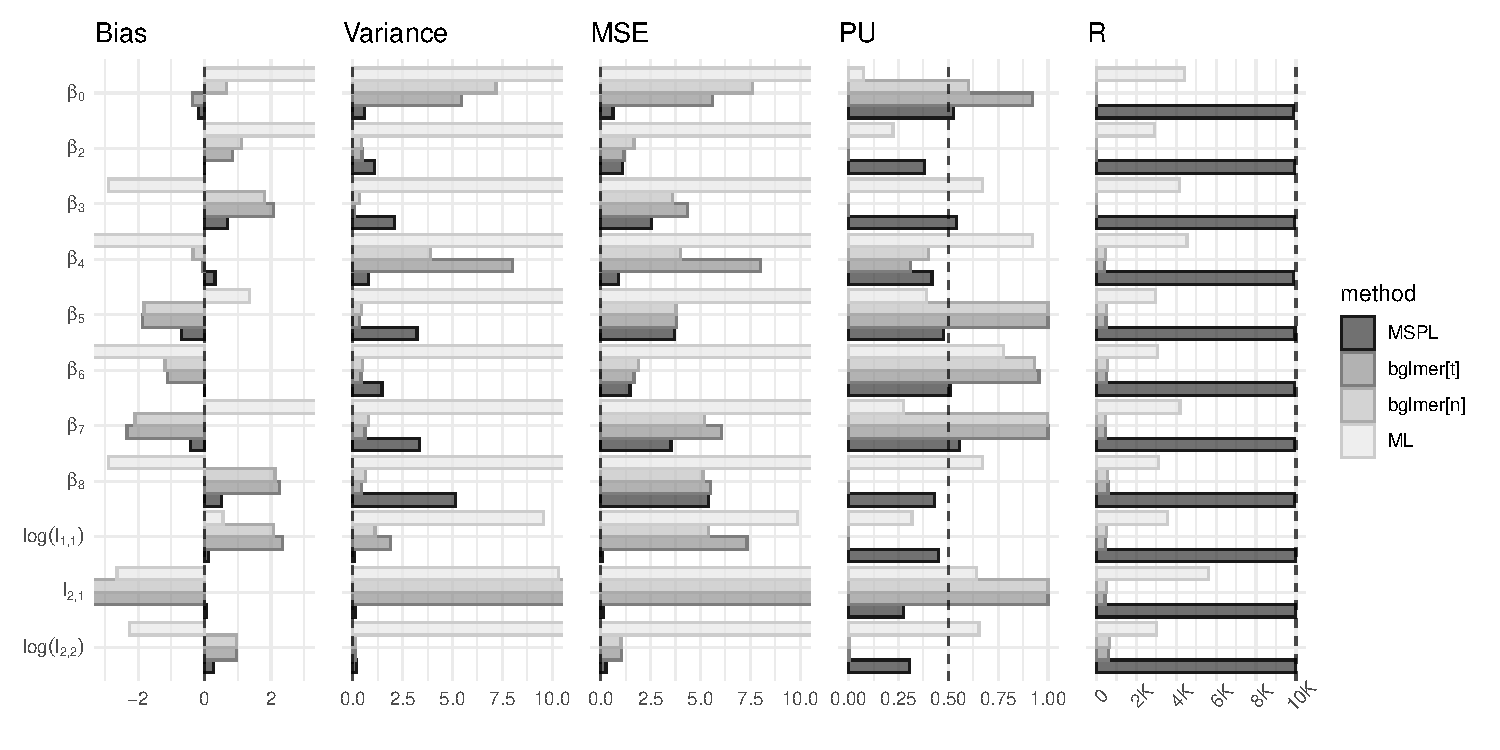
\includegraphics[width=\textwidth]{Figures/cond_inf_simul_full.pdf}
	\caption{Full simulation results from the simulation study in Section 8 of the main text.}
	\label{fig:cond_inf_full}
\end{figure}

\begin{table}[H]
	\centering
	\caption{Percentiles of centred parameter estimates from the simulation study in Section 8 of the main text.}\label{tab:cond_inf_full}
	\begin{tabular}{lrccccccc}
		\toprule 
		&& \multicolumn{7}{c}{Percentiles} \\ \cmidrule{3-9} 
		&&$5\%$&$10\%$&$25\%$&$50\%$&$75\%$&$90\%$&$95\%$\\ \cmidrule{3-9} 
		\cmidrule{3-9} 
		& $\beta_0$ & -2.17 & -2.03 & -0.01 & -0.00 & 0.02 & 0.13 & 0.27 \\ 
		& $\beta_2$ & -2.18 & -2.17 & -0.00 & 0.00 & 0.00 & 2.17 & 2.18 \\ 
		& $\beta_3$ & -1.07 & -0.87 & -0.65 & -0.00 & 2.17 & 2.18 & 2.18 \\ 
		& $\beta_4$ & -0.60 & -0.46 & -0.21 & 0.11 & 0.52 & 1.88 & 2.31 \\ 
		& $\beta_5$ & -4.35 & -2.18 & -2.17 & 0.00 & 0.66 & 1.08 & 2.18 \\ 
		MSPL & $\beta_6$ & -2.30 & -1.56 & -0.51 & -0.00 & 0.52 & 1.62 & 2.30 \\ 
		& $\beta_7$ & -3.27 & -2.73 & -1.84 & -0.23 & 0.78 & 1.68 & 2.82 \\ 
		& $\beta_8$ & -3.24 & -2.35 & -0.96 & 0.41 & 2.05 & 3.39 & 4.31 \\ 
		& $\log l_{1,1}$ & -0.06 & -0.05 & -0.02 & 0.01 & 0.12 & 0.44 & 0.66 \\ 
		& $l_{2,1}$ & -0.66 & -0.27 & -0.02 & 0.12 & 0.21 & 0.35 & 0.45 \\ 
		& $\log l_{2,2}$ & -0.42 & -0.31 & -0.08 & 0.26 & 0.58 & 0.87 & 1.02 \\ 
		\cmidrule{3-9} 
		& $\beta_0$ & -0.88 & -0.86 & -0.80 & -0.50 & 0.06 & 3.26 & 4.33 \\ 
		& $\beta_2$ & 0.17 & 0.22 & 0.46 & 1.31 & 1.61 & 1.85 & 1.88 \\ 
		& $\beta_3$ & 1.17 & 1.20 & 1.41 & 1.74 & 2.09 & 2.57 & 2.73 \\ 
		& $\beta_4$ & -4.37 & -3.96 & -0.65 & 0.24 & 1.01 & 1.51 & 1.79 \\ 
		& $\beta_5$ & -3.11 & -2.79 & -2.17 & -1.72 & -1.37 & -1.09 & -0.87 \\ 
		bglmer[t] & $\beta_6$ & -2.15 & -1.99 & -1.69 & -1.31 & -0.78 & -0.19 & 0.05 \\ 
		& $\beta_7$ & -3.59 & -3.19 & -2.68 & -2.09 & -1.50 & -0.97 & -0.72 \\ 
		& $\beta_8$ & 0.92 & 1.18 & 1.55 & 2.07 & 2.58 & 3.07 & 3.46 \\ 
		& $\log l_{1,1}$ & 1.05 & 1.19 & 1.40 & 1.80 & 2.04 & 4.23 & 4.60 \\ 
		& $l_{2,1}$ & -39.24 & -34.03 & -3.87 & -2.86 & -1.63 & -1.06 & -0.84 \\ 
		& $\log l_{2,2}$ & 0.43 & 0.55 & 0.73 & 0.94 & 1.16 & 1.36 & 1.51 \\ 
		\cmidrule{3-9} 
		& $\beta_0$ & -2.20 & -1.71 & -1.29 & -0.72 & -0.24 & -0.22 & 2.65 \\ 
		& $\beta_2$ & 0.22 & 0.29 & 0.51 & 0.87 & 1.19 & 1.37 & 1.44 \\ 
		& $\beta_3$ & 1.77 & 1.81 & 1.88 & 2.03 & 2.19 & 2.41 & 2.51 \\ 
		& $\beta_4$ & -5.50 & -4.93 & -1.17 & 1.04 & 1.99 & 2.51 & 2.69 \\ 
		& $\beta_5$ & -2.82 & -2.51 & -2.20 & -1.82 & -1.49 & -1.19 & -1.01 \\ 
		bglmer[n] & $\beta_6$ & -2.12 & -1.91 & -1.59 & -1.12 & -0.69 & -0.30 & -0.05 \\ 
		& $\beta_7$ & -3.65 & -3.26 & -2.83 & -2.31 & -1.84 & -1.40 & -1.09 \\ 
		& $\beta_8$ & 1.23 & 1.44 & 1.80 & 2.25 & 2.66 & 3.12 & 3.31 \\ 
		& $\log l_{1,1}$ & 0.95 & 1.04 & 1.21 & 1.91 & 3.81 & 4.55 & 4.92 \\ 
		& $l_{2,1}$ & -38.54 & -34.65 & -4.03 & -2.73 & -1.29 & -0.92 & -0.78 \\ 
		& $\log l_{2,2}$ & 0.44 & 0.58 & 0.74 & 0.95 & 1.16 & 1.36 & 1.52 \\ 
		\cmidrule{3-9} 
		& $\beta_0$ & -1.11 & 1.58 & 5.84 & 9.60 & 11.76 & 13.58 & 14.87 \\ 
		& $\beta_2$ & -8.42 & -7.29 & 0.76 & 4.96 & 7.59 & 10.71 & 12.75 \\ 
		& $\beta_3$ & -10.06 & -8.74 & -7.04 & -5.40 & 2.16 & 5.85 & 9.43 \\ 
		& $\beta_4$ & -14.59 & -13.43 & -11.64 & -9.51 & -5.65 & -1.42 & 1.28 \\ 
		& $\beta_5$ & -10.07 & -6.58 & -1.34 & 0.74 & 2.89 & 8.63 & 16.11 \\ 
		ML & $\beta_6$ & -12.92 & -10.61 & -7.41 & -4.88 & -1.04 & 7.29 & 8.40 \\ 
		& $\beta_7$ & -6.77 & -5.02 & -0.91 & 5.61 & 7.60 & 10.38 & 13.80 \\ 
		& $\beta_8$ & -19.81 & -11.80 & -5.30 & -1.21 & 0.80 & 3.99 & 8.77 \\ 
		& $\log l_{1,1}$ & -2.75 & -2.05 & -0.91 & 1.21 & 2.36 & 2.62 & 2.66 \\ 
		& $l_{2,1}$ & -7.47 & -7.19 & -5.74 & -1.51 & 0.54 & 0.81 & 1.09 \\ 
		& $\log l_{2,2}$ & -6.62 & -4.54 & -3.22 & -1.77 & 0.39 & 0.85 & 1.04 \\ 
		\bottomrule 
	\end{tabular}
\end{table}


\section{Further Simulations} \label{sec:simuls}

\subsection{Simulation 1: Extreme fixed effects}\label{sec:sim1}

This section presents a simulation that seeks to provoke degenerate fixed effects estimates through a strong dependence of the responses on the particular fixed effects -- a phenomenon known to occur in standard logistic regression \citep{albert+anderson:1984,kosmidis+firth:2021}.

For this, we simulate from a mixed effects logistic regression with univariate random effects and logistic link function as follows. For five clusters $i=1,\ldots,5$ and within cluster observations $j=1,\ldots,n$, $n \in \{50,100,200\}$, we draw an i.i.d. vector of fixed effects covariates $\bx_{ij} = (x_{i1},x_{i2},x_{i3},x_{i4},x_{i5})$ where $X_{i1}=1, {X}_{i2} \sim \text{N}(0,1), {X}_{i3}\sim \textrm{Ber}\left(\frac{1}{2}\right), {X}_{i4}\sim~\textrm{Ber}\left(\frac{1}{4}\right)$, and ${X}_{i5}\sim~\exp(1)$. The fixed effect covariates are drawn once and held fixed over the simulation. To control the degree of dependence of the responses on a particular fixed effect covariate, the parameter of fixed effects is set as $\bb \beta=(1,-0.5,\lambda,0.25,-1)$, where $\lambda$ takes integer values from $-10$ to $10$. For each specification of $n$, $\lambda$, we draw 100 samples from the model 
\begin{equation}
	\begin{aligned}
		\label{eq:sim1_model} 
		Y_{ij} \mid {u}_i & \sim \text{Bernoulli}(\mu_{ij}) \quad \text{with} \quad
		g(\mu_{ij}) = \eta_{ij} = \bx_{ij}^\top \bb \beta + u_i,\\
		u_i & \sim \text{N}(0, 9)  \quad (i = 1, \ldots, 5; j = 1, \ldots, n), \quad n\in \{50,100,200\}
	\end{aligned}
\end{equation}
The random effects dispersion parameter $\sigma = 3$ was chosen as to avoid estimation issues associated with small random effects. We estimate the parameters using our proposed MSPL with the penalties given in Section 5 of the main text, ML and \texttt{bglmer}  from the \texttt{blme} R \citep{R} package \citep{chung+etal:2013} with a normal and t prior for the fixed effects and a gamma prior for the random effects variance. We approximate the log-likelihood with a 20-point adaptive Gauss-Hermite quadrature approximation. For ML and MSPL, we optimize the approximate log-likelihood using the optimization methods ``CG'', ``BFGS'', ``nlminb'' and ``L-BFGS-B'' from the \texttt{optimx} R package \citep{nash:2014} and report the best fit. Both \texttt{bglmer} specifications use the default \texttt{bglmer} optimization settings. 

Table \ref{tab:sim1} shows the number of estimates per specification which resulted in an degenerate parameter estimate. We considered an estimate degenerate, if it is larger than $50$ in absolute value, the gradient is larger than $0.001$ in absolute value, or if the estimated asymptotic standard errors are larger than $40$. Figure \ref{fig:sim1} shows the dispersion of the estimates ${\beta}_3$ around the true value (indicated by dashed horizontal line) per specification for all estimation methods. For presentability, the y-axis has been cropped to omit overly extreme estimates. For the ML, 672 estimates are cropped, while  for all other methods, all estimates are shown. Note that the boxplots for the ML do not depict the empirical distribution of the ML estimate of $\beta_3$ over different samples as theoretically infinite estimates assume finite values in estimation due to numerical precision limitations and resulting premature declaration of convergence. We see from Table \ref{tab:sim1} that the MSPL gives the most stable parameter estimation, with one out of 6000 samples exhibiting estimation issues due to failed convergence. The ML on the other hand becomes highly problematic for large values of $\beta_3$ and even returns degenerate estimates for moderate values of $\beta_3$ with non-negligible frequency. The \texttt{bglmer} estimates, even though they penalize fixed effects more harshly, as can be seen by the shrinkage-induced bias of the \texttt{bglmer} estimates of $\beta_3$ in Figure \ref{fig:sim1}, they encounter estimation issues substantially more often than the MSPL estimates. 
\begin{figure}[H]
	\begin{center}
		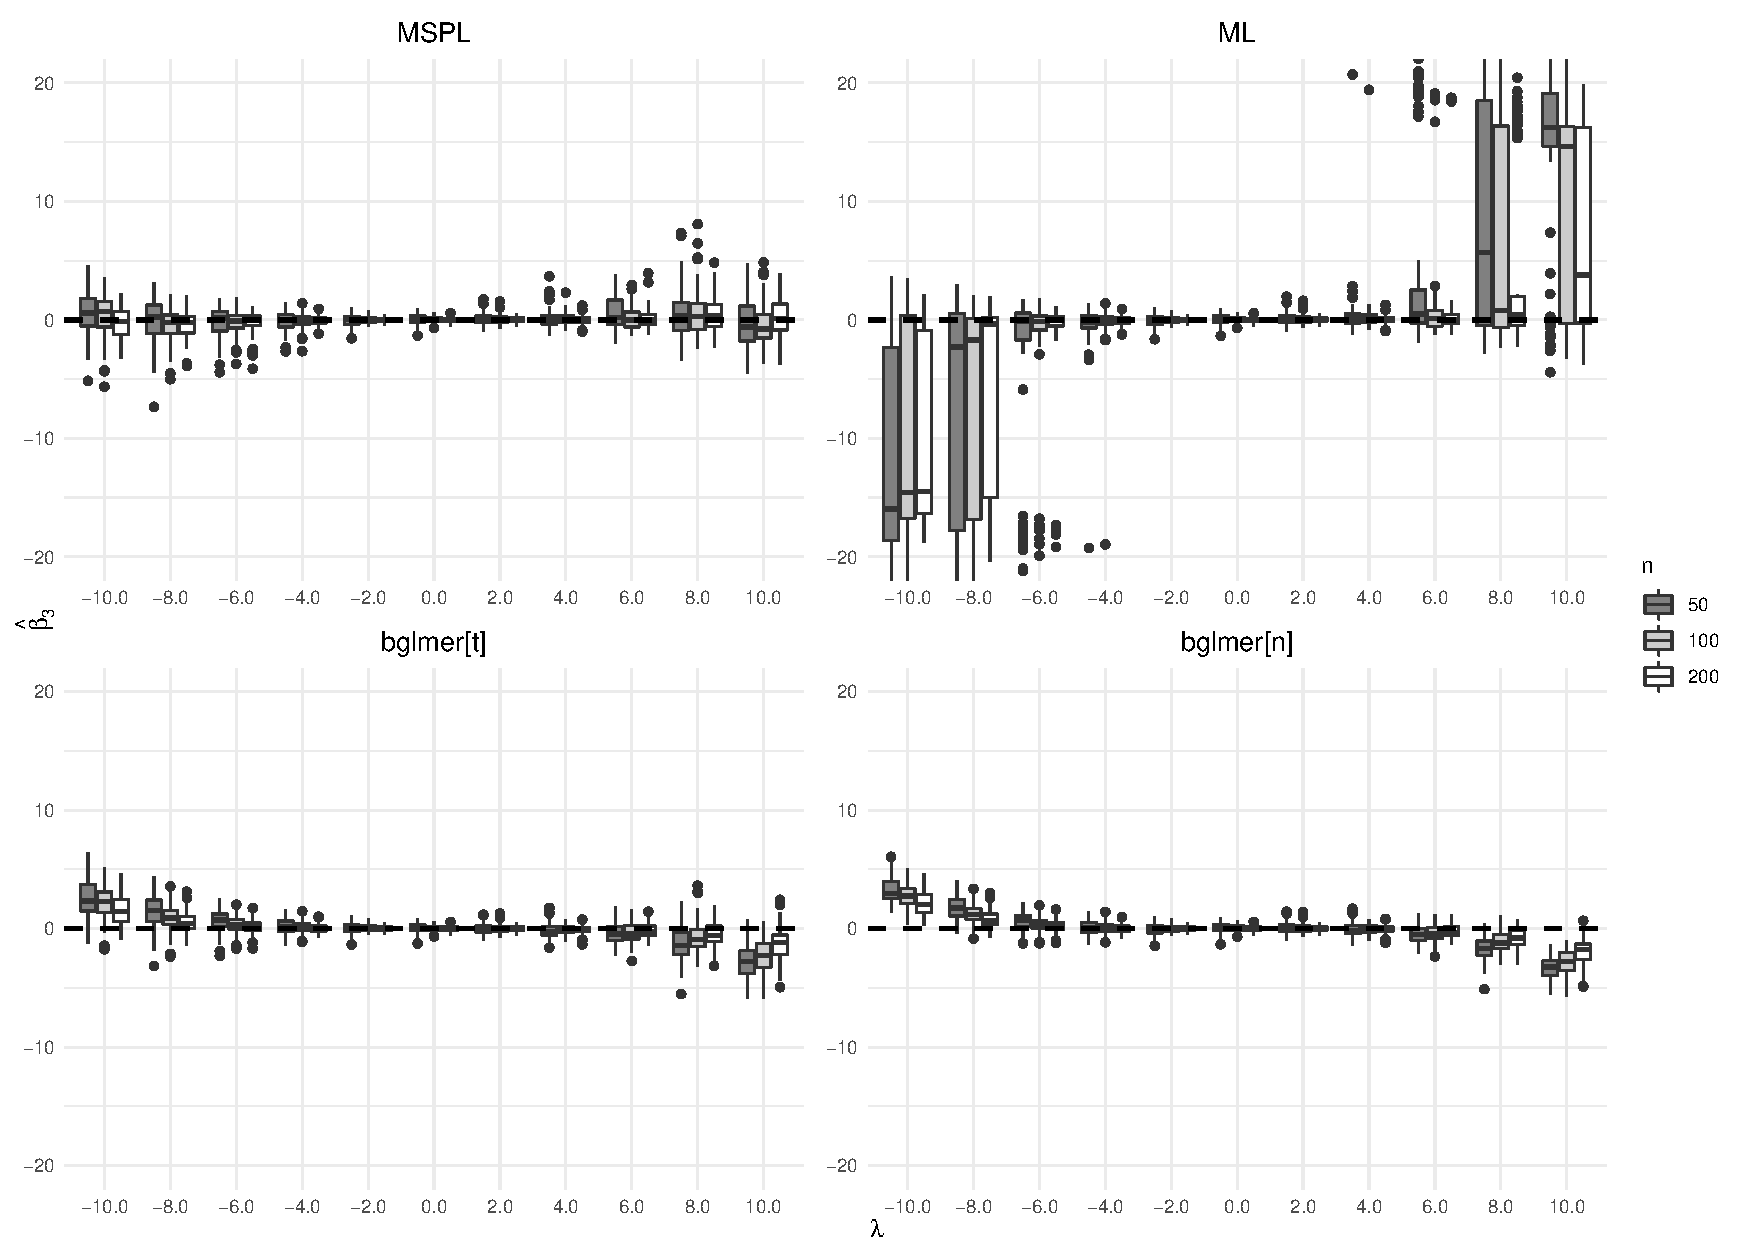
\includegraphics[width=\textwidth]{Figures/sim1.pdf}
	\end{center}
	\caption{Centered estimation output of $\beta_3$ from Simulation \hyperref[sec:sim1]{1}}
	\label{fig:sim1}
\end{figure}

\begin{table}[H]
	\centering
	\caption{Percentage of degenerate estimates from Simulation \hyperref[sec:sim1]{1}} 
	\label{tab:sim1}
	\begin{tabular}{lrccccccccccc}
		\toprule 
		&& \multicolumn{11}{c}{$\lambda$} \\ \cmidrule{3-13} 
		&  & -10 & -8 & -6 & -4 & -2 & 0 & 2 & 4 & 6 & 8 & 10 \\ 
		\cmidrule{3-13} 
		& n=50 & 0 & 0 & 0 & 0 & 0 & 0 & 0 & 0 & 0 & 0 & 0 \\ 
		MSPL & n=100 & 0 & 0 & 0 & 0 & 0 & 0 & 0 & 0 & 0 & \textbf{1} & 0 \\ 
		& n=200 & 0 & 0 & 0 & 0 & 0 & 0 & 0 & 0 & 0 & 0 & 0 \\ 
		\cmidrule{3-13} 
		& n=50 & \textbf{73} & \textbf{46} & \textbf{17} & \textbf{2} & 0 & 0 & 0 & \textbf{1} & \textbf{15} & \textbf{49} & \textbf{80} \\ 
		ML & n=100 & \textbf{63} & \textbf{45} & \textbf{10} & \textbf{1} & 0 & 0 & 0 & \textbf{1} & \textbf{5} & \textbf{31} & \textbf{61} \\ 
		& n=200 & \textbf{65} & \textbf{26} & \textbf{8} & 0 & 0 & 0 & 0 & 0 & \textbf{2} & \textbf{24} & \textbf{49} \\ 
		\cmidrule{3-13} 
		& n=50 & 0 & 0 & 0 & 0 & 0 & 0 & 0 & 0 & 0 & 0 & 0 \\ 
		bglmer[t] & n=100 & 0 & 0 & 0 & \textbf{1} & 0 & 0 & 0 & 0 & 0 & 0 & 0 \\ 
		& n=200 & 0 & 0 & \textbf{1} & 0 & \textbf{1} & 0 & 0 & 0 & 0 & 0 & \textbf{1} \\ 
		\cmidrule{3-13} 
		& n=50 & \textbf{1} & 0 & 0 & 0 & 0 & \textbf{1} & 0 & 0 & 0 & 0 & 0 \\ 
		bglmer[n] & n=100 & 0 & 0 & \textbf{1} & 0 & \textbf{1} & 0 & 0 & 0 & \textbf{1} & 0 & 0 \\ 
		& n=200 & 0 & 0 & 0 & 0 & 0 & 0 & 0 & 0 & 0 & 0 & 0 \\ 
		\bottomrule 
	\end{tabular}
\end{table}



\subsection{Simulation 2: Extreme random effects variance} \label{sec:sim2}
In this simulation, we seek to provoke degenerate random effects variance estimates, that is random effects variance estimates that are either zero or infinite. One of the peculiarities of Bernoulli-response (or Binomial-response) mixed effects models is that there can be separation of the observations with respect to the random effects covariates. Analogously to separation in logistic regression models \citep{albert+anderson:1984}, where covariate constellations such that the responses can be separated by a hyperplane spanned by the covariate column vectors, lead to infinite parameter estimates, it is known that certain constellations of random effects covariates can lead to data separation and consequently degenerate random effects estimates (see for example \citet{sauter+held:2016} or the discussion on \url{https://stats.stackexchange.com/questions/44755}). We consider a simple simulation to provoke such data configurations by simulating from a mixed effects logistic regression with univariate random effects and vary the dependence of the responses on the grouping variable by controlling the random effects variance parameter. 

For five clusters $i=1,\ldots,5$ and within cluster observations $j=1,\ldots,n$, $n \in \{50,100,200\}$, we draw an i.i.d. vector of fixed effects covariates $\bx_{ij} = (x_{i1},x_{i2},x_{i3},x_{i4},x_{i5})$ where $X_{i1}=~1$, ${X}_{i2} \sim \text{N}(0,1), {X}_{i3}\sim \textrm{Ber}\left(\frac{1}{2}\right), {X}_{i4}\sim~\textrm{Ber}\left(\frac{1}{4}\right)$, and ${X}_{i5}\sim~\exp(1)$. The fixed effect covariates are drawn once and held fixed over the simulation. Likewise, the fixed effects $\bb \beta  =~(1,-0.5,0.5,0.25,-1)$ are held fixed over the simulation, while $\lambda = \log \sigma$ is varied  over the integer values from $-5$ to $2$. For each specification of $n$, $\lambda$, we draw 100 samples from the model 
\begin{equation}
\begin{aligned}
\label{eq:sim2_model} 
Y_{ij} \mid {u}_i & \sim \text{Bernoulli}(\mu_{ij}) \quad \text{with} \quad
g(\mu_{ij}) = \eta_{ij} = \bx_{ij}^\top \bb \beta + u_i,\\
u_i & \sim \text{N}(0, \exp (\lambda)^2 )  \quad (i = 1, \ldots, 5; j = 1, \ldots, n), \quad n\in \{50,100,200\}
\end{aligned}
\end{equation}
We estimate the parameters using our proposed MSPL with the penalties given in Section 6 of the main text, ML and \texttt{bglmer}  from the \texttt{blme} R package \citep{chung+etal:2013} with a normal and t prior for the fixed effects and a gamma prior for the random effects variance. We approximate the log-likelihood with a 20-point adaptive Gauss-Hermite quadrature approximation. For ML and MSPL, we optimize the approximate log-likelihood using the optimization methods ``CG'', ``BFGS'', ``nlminb'' and ``L-BFGS-B'' from the \texttt{optimx} R package \citep{nash:2014} and report the best fit. Both \texttt{bglmer} specifications use the default \texttt{bglmer} optimization settings. Figure \ref{fig:sim2} shows the dispersion of the estimates for $\log \sigma$ around the true value (indicated by dashed horizontal line), for each estimation method and specification of $\lambda ,n$. For the ML and \texttt{bglmer} estimates, these boxplots do not approximate the distribution of the maximum likelihood estimator as, owed to numerical precision limitations, parameter estimates which ought to be infinite or zero are not estimated as such so that the point masses at the boundaries of the parameter space are missing. For bglmer[t], 6 estimates are not shown and for bglmer[n], 4 estimates are not shown due to failed estimation. While both the MSPL and \texttt{bglmer} shrink negative estimates of $\log \sigma$ towards zero, the shrinkage induced by \texttt{bglmer} is considerably stronger, as can be seen by the absolute amount of shrinkage and the smaller dispersion of the estimates. Moreover, we see that for larger values of $\log \sigma$ \texttt{bglmer} is unable to guard against infinite estimates of the random effects variance. 

Table \ref{tab:sim2} shows the number of estimates for $\log \sigma$ per specification which resulted in an degenerate random effects variance estimate. We considered an estimate degenerate, if it is larger than $\log(50)$ or smaller than $\log(0.01)$, the gradient is larger than $0.001$ in absolute value, or if the estimated asymptotic standard errors are larger than $40$. We see that MSPL is the most stable estimation routine and that both \texttt{bglmer} and ML exhibit estimation degeneracies frequently for both small and large values of the random effects variance. 
\begin{figure}[H]
	\begin{center}
		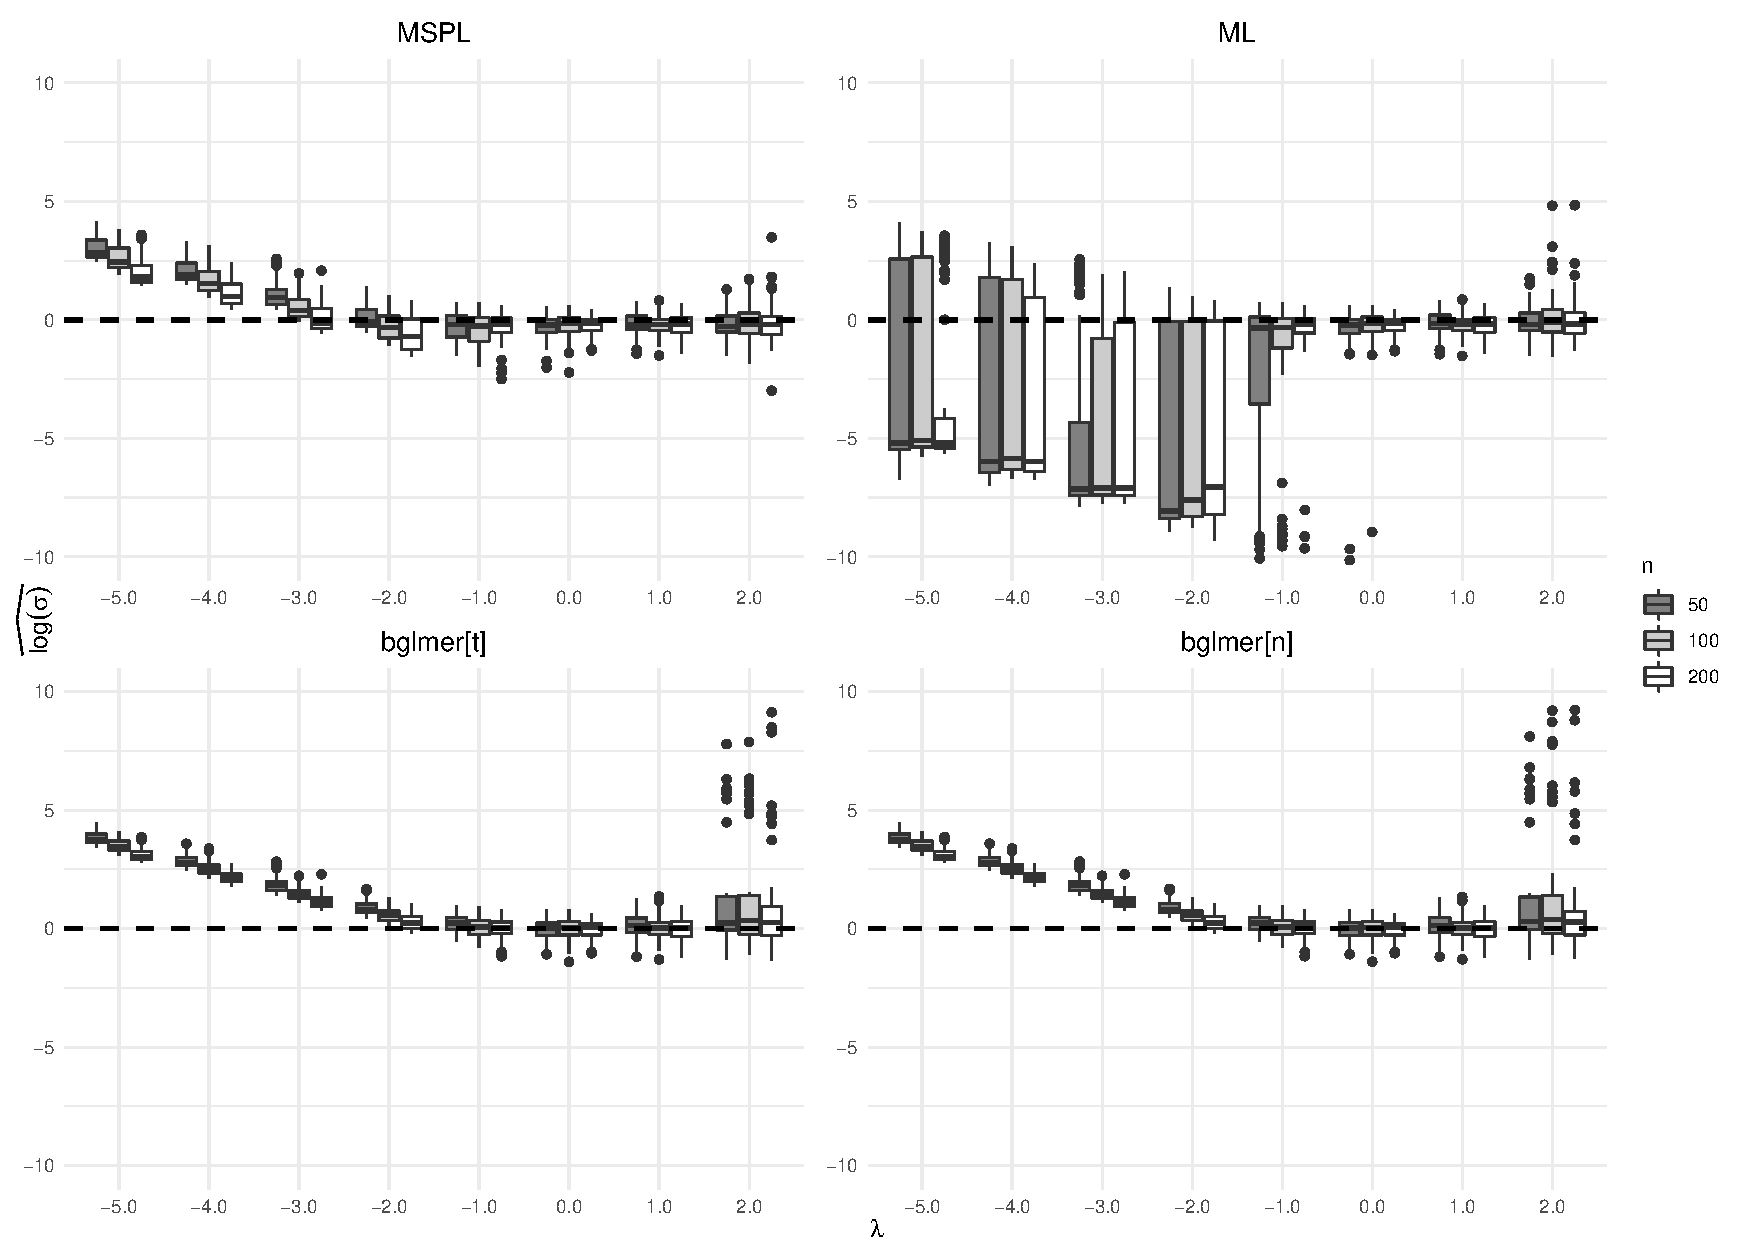
\includegraphics[width=\textwidth]{Figures/sim2.pdf}
	\end{center}
	\caption{Centered estimation output of $\log \sigma$ from Simulation \hyperref[sec:sim2]{2}}
	\label{fig:sim2}
\end{figure}

\begin{table}[H]
	\centering
	\caption{Percentage of degenerate estimates from Simulation \hyperref[sec:sim2]{2}} 
	\label{tab:sim2}
	\begin{tabular}{lrcccccccc}
		\toprule 
		&& \multicolumn{8}{c}{$\lambda$} \\ \cmidrule{3-10} 
		&  & -5 & -4 & -3 & -2 & -1 & 0 & 1 & 2 \\ 
		\cmidrule{3-10} 
		& n=50 & 0 & 0 & 0 & 0 & 0 & 0 & 0 & \textbf{1} \\ 
		MSPL & n=100 & 0 & 0 & 0 & 0 & 0 & 0 & 0 & 0 \\ 
		& n=200 & 0 & 0 & 0 & 0 & 0 & 0 & 0 & \textbf{2} \\ 
		\cmidrule{3-10} 
		& n=50 & \textbf{73} & \textbf{70} & \textbf{76} & \textbf{70} & \textbf{25} & \textbf{2} & 0 & 0 \\ 
		ML & n=100 & \textbf{68} & \textbf{68} & \textbf{75} & \textbf{58} & \textbf{16} & \textbf{1} & 0 & \textbf{7} \\ 
		& n=200 & \textbf{78} & \textbf{68} & \textbf{69} & \textbf{52} & \textbf{4} & 0 & 0 & \textbf{5} \\ 
		\cmidrule{3-10} 
		& n=50 & 0 & 0 & 0 & 0 & 0 & 0 & 0 & \textbf{12} \\ 
		bglmer[t] & n=100 & \textbf{2} & \textbf{2} & \textbf{6} & \textbf{3} & \textbf{3} & 0 & 0 & \textbf{17} \\ 
		& n=200 & \textbf{26} & \textbf{35} & \textbf{23} & \textbf{15} & \textbf{4} & 0 & 0 & \textbf{11} \\ 
		\cmidrule{3-10} 
		& n=50 & 0 & 0 & 0 & 0 & 0 & 0 & 0 & \textbf{12} \\ 
		bglmer[n] & n=100 & \textbf{2} & \textbf{1} & \textbf{2} & 0 & 0 & 0 & 0 & \textbf{17} \\ 
		& n=200 & \textbf{20} & \textbf{22} & \textbf{20} & \textbf{15} & \textbf{3} & 0 & 0 & \textbf{11} \\ 
		\bottomrule 
	\end{tabular}
\end{table}

\bibliographystyle{chicago}
\bibliography{softpen}
\end{document}